\documentclass{article}
\usepackage[utf8]{inputenc}
\usepackage{graphicx}
\usepackage{biblatex}
\addbibresource{ref.bib}

\title{Introdução à Biologia Molecular Computacional \LaTeX}
\author{Talita Giovanna Xavier de Oliveira}
\date{03 de Agosto de 2021}

\begin{document}

\maketitle

\section{Introdução}
\par 
A biologia Molecular computacional nos permite ordenar os resultados gerados das iniciativas de sequenciamento de genes, ao qual produzem quantidades cada vez maiores de dados sobre sequências de DNA e seus produtos proteicos, através da manipulação e análise de dados biológicos e problemas da área apresentados. Sendo assim, é possível utilizar métodos estatísticos, em conjunto com uma abordagem computacional, que são capazes de analisar uma grande quantidade de dados biológicos, de inferir funções dos genes e também de estabelecer relações estruturais entre genes e proteínas\cite{araujo}.
\begin{figure}[ht]
    \centering
    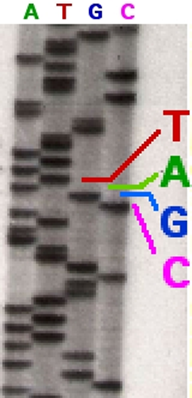
\includegraphics[scale= 0.2]{DNA seq.png}
    \caption{Imagem de uma parte de um gel de sequenciamento radioativo marcado\cite{biologia}}
    \label{imagem_um}
\end{figure}
\begin{figure}[ht]
    \centering
    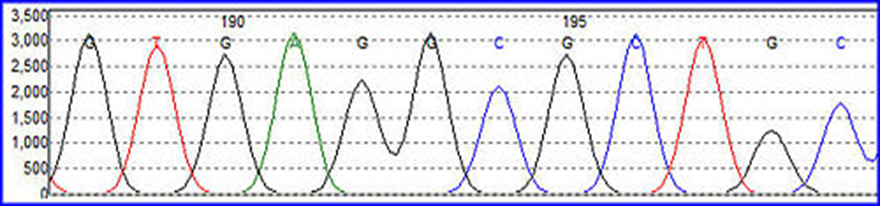
\includegraphics[scale= 0.2]{DNA sequenciamento.png}
    \caption{Imagem de um sequenciamento de DNA\cite{biologia}}
    \label{imagem_dois}
\end{figure}
\section{Relevância}
\par 
Devido ao avanço da humanidade ao longo dos anos fazendo com que pesquisas científicas se tornassem mais complexas e a enorme quantidade de dados, tornou-se necessário o surgimento de uma nova ferramenta para dar conta da  por espaço de armazenamento e análise de dados, além de auxiliar o crescimento constante da ciência. E a área de biologia molecular computacional é uma das mas conhecidas e responsável por impulsionar a bio-informática.
\par 
Um exemplo de aplicação da biologia molecular computacional é a identificação de alvos proteicos que tem potencial para serem modificados diretamente pela interação com os fármacos podendo minimizar os sintomas ou as causas de algumas doenças, além de também permitir a detecção molecular de parasitas, levando diretamente no diagnóstico e na epidemiologia de diversas patologias\cite{araujo}.
\section{Relações com outras disciplinas}
\par
As relações da biologia molecular computacional com outras disciplinas é extremamente ilimitada por ser uma área de estudo interdisciplinar, ao qual trabalha tanto com uso da área de tecnologia, quanto da área de exatas e saúde\cite{ementa}.
\par
É uma disciplina eletiva ao qual faz parte do perfil de bioinformática do curso de Ciências da Computação tendo ligação com a disciplina da pós-graduação IN1115 - Introdução à Bio-informática e biologia computacional, não apresentando pré-requisito e nem có-requisito e tendo equivalência apenas com a disciplina IF130 - Teoria dos Modelos\cite{ementa}. 

\printbibliography
\end{document}
